\chapter{Project Focus}
This report is centered about Parental Control (PC) in Smart Home (SH). This chapter will explain what PC and SH is, as well as explorer a field of different possibilities and narrow the possibilities down to a reasonable amount of goals for this project.

%What is smart home
\section{Smart Home}
A Smart Home can refer to multiple forms of improvement on a home. Most commonly is home automation, environment friendly improvements and power saving improvements. In this report we will only regard Smart Home in relation to home automation, however environment friendly- and power saving improvements, sometimes also springs out of home automation. For example if you automate the washing machine to start at a certain hour of the day, it will both be convenient as well as power saving.\\
\\
But a Smart Home, can be much more. Different examples of implementable features is as follows:

\begin{itemize}
	\item Automated security
	\item Music systems
	\item Theater systems
	\item Voice commands
	\item Automatic ordering of groceries
	\item Delayed start on an oven
	\item Automated coffee machines
	\item Light control
	\item Power control on leaving home
	\item And much more
\end{itemize}

This report is about a less common feature of a Smart Home. It is about Parental Control, a concept explained in \ref{parentalControl}.

%What is parental control
\section{Parental Control}
\label{parentalControl}
Parental Control (PC) is a concept most people know from their TV at home or computers. A concept used mainly by parents to protect their children from fx. internet sites with adult content or TV channels of the same kind.\\
But in a Smart Home, this concept could be taken even further. Many electronic devises does not implement a PC feature, and some of those which does, does not allow to block all content.\\
We want to create a system that could help parents manage their children's time. We want to do this in order to improve the well being of children. Studies show that children of the newer ages are sitting indoors, more and more.\citep{childrenAndNature}\citep{leaveNoChildInside}\\
These studies also tell how staying inside both limits the child’s imagination and is a factor for stress. It has also been linked to an increase in likelihood of these children having ADHD.\\
\\
What this project is aiming at is to create a system that would allow the parents to both, help manage their children's time, as well as encourage them to go outside and play.\\
In order for this to succeed, the implementation must offer this control set, without becoming too much of a bother for both the parents and the children it impacts. We do not want to restrict and limit, but rather organize and encourage. - This effectively means, the system can not impose a too long addition to the start up of the restricted devices and the system must implement a feature for the children to earn more time for the restricted devices. These requirements will be gone into further details at a later point REF...

%Write about the brainstorm we did
\section{Potential of Parental Control}
In order to determine the potential for the Parental Control system, a brainstorm was made, to visualize the ideas and couplings that could be made with an existing Smart Home implementation. For this brainstorm we took the base concept of a Smart Home as introduced by Mi Casa Verde\citep{micasaverde}.


\begin{figure}[htbp]
	\centering
		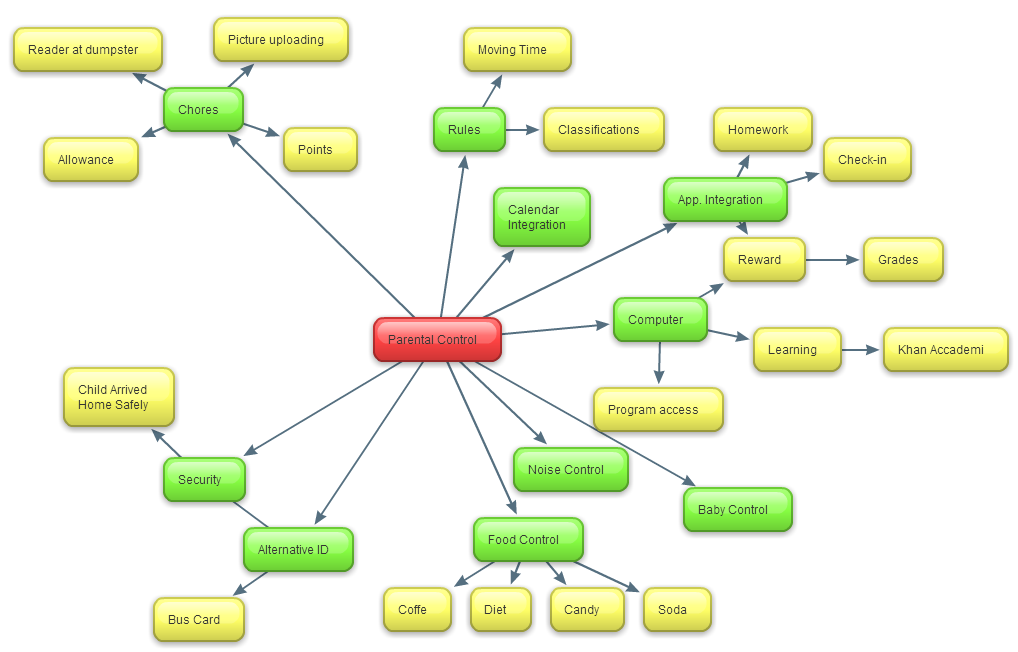
\includegraphics[width=1.50\textwidth]{images/BrainStorm.png}
	\caption{Brainstorm over Parental Control}
	\label{fig:BrainStorm}
\end{figure}

%Explain each point of the Brainstorm, atleast the Green ones, also explain the color codes.
In figure \ref{fig:BrainStorm} is seen 3 different colors. Red is our starting point. Green is our direct sub-points and yellow is our indirect sub-points.\\
Next is a walkthrough of each of the direct sub-points.\\
\subsection{Chores}
The idea of Chores is that a child would be able to do a chore and after doing this chore he would receive a reward in the form of either extra allowance or points that could be spent on more time in front of his electronic devices.\\
The main idea was to let the child do the chore, then tell his parents. The parents then go onto the online admin web interface and accepts that the chore is done. Other ideas of how to accept a chore was done, was to let the child upload an image of what they had done, this would give the parents a notification, and they could then check if it was done.\\
Another suggestion was to put a reader outside of the dumpster, or at other convenient positions, relating to a chore. - This would however need a little extra thinking over if it is not to be abused.

\subsection{Rules}
This is simply an extra implementation to the admin web interface. It relates to a few settings available for the parents and what features must be considered for the system to function.\\
One feature that needed special consideration is if it possible to save ''time-points'' from week to week.\\
Another is how classes is implemented, especially how we consider both parents and children. And also in this relation how we consider different devices plugged into this system.

\subsection{Calendar Integration}
Simple as it sounds, calendar integration would require a great deal of thinking over. The idea of the feature is to let the parents hook up a calendar to the system, for each child. Then if the parents put an event into the calendar, they can force the shut down of any devices used by the child in due time for the child to get ready for the event.\\
On the other hand it could also be possible to put in events that allowed the child to play the whole day.

\subsection{App. Integration}
This is the idea of creating an application for mobile devices as well as the web interface.
There is multiple parts to this idea. First there is the idea to let the child use this app to make a ''check-in'' so that his parents know he went where he was supposed to, and that he is safe. He would then be remembered to this check in once in a while. If he failed to check-in a notification would be sent to his parents.\\
Secondly, there is the idea to let other grownups reward the child with points, if they do a good deed. For example if they came to soccer practice and worked extra hard at it.\\
The third idea was to let it be implemented into a school system. Allowing the teacher to give homework, or notes through the system. Then homework could be rewarding x points.

\subsection{Computer}
The main idea is to let the child log in through the Smart Home Parental Control system. Here it should then be possible to specify certain deeds that could be done on the computer, for example playing an educational game, would result in more time on the computer.\\
Also in order not to take away the child's play time, it would be needed to monitor if the child was actively researching or writing. If this is not the case, the system should start to count time usage.\\
The system could also be used to restrict the usage of programs, both in periodic measures, or permanently. This way the parents can have a program not accessible for the child.

\subsection{Noise Control}
The idea is to implement a feature in all audio devices that the system should be hooked up to, that prevents the raising of the volume to a certain point. - This could again be made into a permanent effect or an effect that only was in effect for periods of time.

\subsection{Baby Control}
The idea came up in relation with the app. integration idea. The idea was to let the system monitor a baby and if a certain screaming noise was heard, or if the infrared reading of the child was gone, it would send a message to the parent.

\subsection{Food Control}
The idea sprung out of the relation of children welfare. The idea was to put a lock on cupboards, that would require the child to open it with its key. This way, parents could make sure the child is not eating between meals if not allowed.\\
Another idea was to somehow monitor the amount of soda a child was allowed to drink each week.\\
A third idea was to help the parents, not drinking too much coffee. By requiring them to use their key, to make the coffee machine make coffee. This way the parent could enter a certain amount of cups that he would be allowed to drink on a normal day. Of course with the ability to shut this feature of as needed.

\subsection{Alternative ID and Security}
This idea sprung out of the idea that the child would be carrying a digital key with them constantly. If this was the case, it could maybe be used for opening the door at home, giving the possibility of giving the parents a notification about their child arriving safely home from school.\\
Or maybe as an access card for the school, or the school bus.\\
It could also contain relevant information in the event of an accident. For example what illnesses the child has and contact information of the parents.\\
\\
All these features do however demand a level of security and encryption to be taken into account.

%Narrow down the area we want to covor
\section{Finding the project focus}
Given the above walkthrough of ideas, it is clear that the system could be implemented to contain many features. But the implementation would take time, more time than a project group at Aalborg University has for one semester. Therefore we must narrow down the field of implementation.\\
\\
%Specify what must be done, in order for it to succed
In order for the system to implemented there must be created a device, that can use some sort of personalized key, to activate the powersupply for the electronic devices that the parents wants to restrict.\\
There must also be created a configurable set of rules, that preferably could be accessed from the internet, to open up for the most features.\\
\\
This project is about proof of concept. Therefore the focus will lay in the most central features. This means that Alternative ID, Security, Food Control, Noise Control and Baby Control is the least important since all these ideas are not concerned with helping to get the child away from IT/TV systems.\\
That leaves Computer, App. Integration, Calendar Integration, Rules and Chores.\\
A core concept is Chores and Rules, since they allow for the child to earn points, and would fit into the Smart Home concept.
Next Calendar Integration would be a tool that could be used for children in all ages. Since this does not require the child to have a calendar of their own, rather their parents can administer one for them.\\
After these three, comes App. Integration and Computer on an equal level. The App. Integration would open up for the possibility of helping parents know where their children are when the child is old enough to have their own smart phone. As well as being a way to gather more points from sport activities.\\
Computer would again open up for another way of collecting points and it has the potential to motivate the children to study.\\
\\
This means that in prioritized order, this project will focus on implementing these features: Rules, Chores, Calendar Integration, App. Integration and Computer.